%% Wraparound paperback cover for KDP
%% Trim 7 x 10 in, 0.125 in bleed on all sides, spine width from page count (white paper).
\documentclass{article}
\def\spinewidth{1.1012}
  % defines \spinewidth (in inches, a number)
\usepackage[T1]{fontenc}
\usepackage{mathpazo}
\usepackage{tikz}
\usepackage{xcolor}
\usetikzlibrary{calc}

\newlength{\bleed}\setlength{\bleed}{0.125in}
\newlength{\trimw}\setlength{\trimw}{7in}
\newlength{\trimh}\setlength{\trimh}{10in}
\newlength{\spine}\setlength{\spine}{\spinewidth in}
\newlength{\coverw}\setlength{\coverw}{\dimexpr 2\bleed + 2\trimw + \spine\relax}
\newlength{\coverh}\setlength{\coverh}{\dimexpr 2\bleed + \trimh\relax}
\usepackage[paperwidth=\coverw,paperheight=\coverh,margin=0pt]{geometry}

\definecolor{navy}{HTML}{13233A}
\definecolor{navyb}{HTML}{1B3050}
\definecolor{gold}{HTML}{D9A441}
\definecolor{cream}{HTML}{F3EBDD}
\definecolor{rust}{HTML}{B5543A}
\definecolor{sage}{HTML}{8FA88A}
\definecolor{teal}{HTML}{3E7C87}
\tikzset{treeline/.style={draw=gold!85!cream, line width=0.7pt, line cap=round, line join=round}}

\pagestyle{empty}
\hyphenpenalty=10000
\exhyphenpenalty=10000
\begin{document}
\noindent
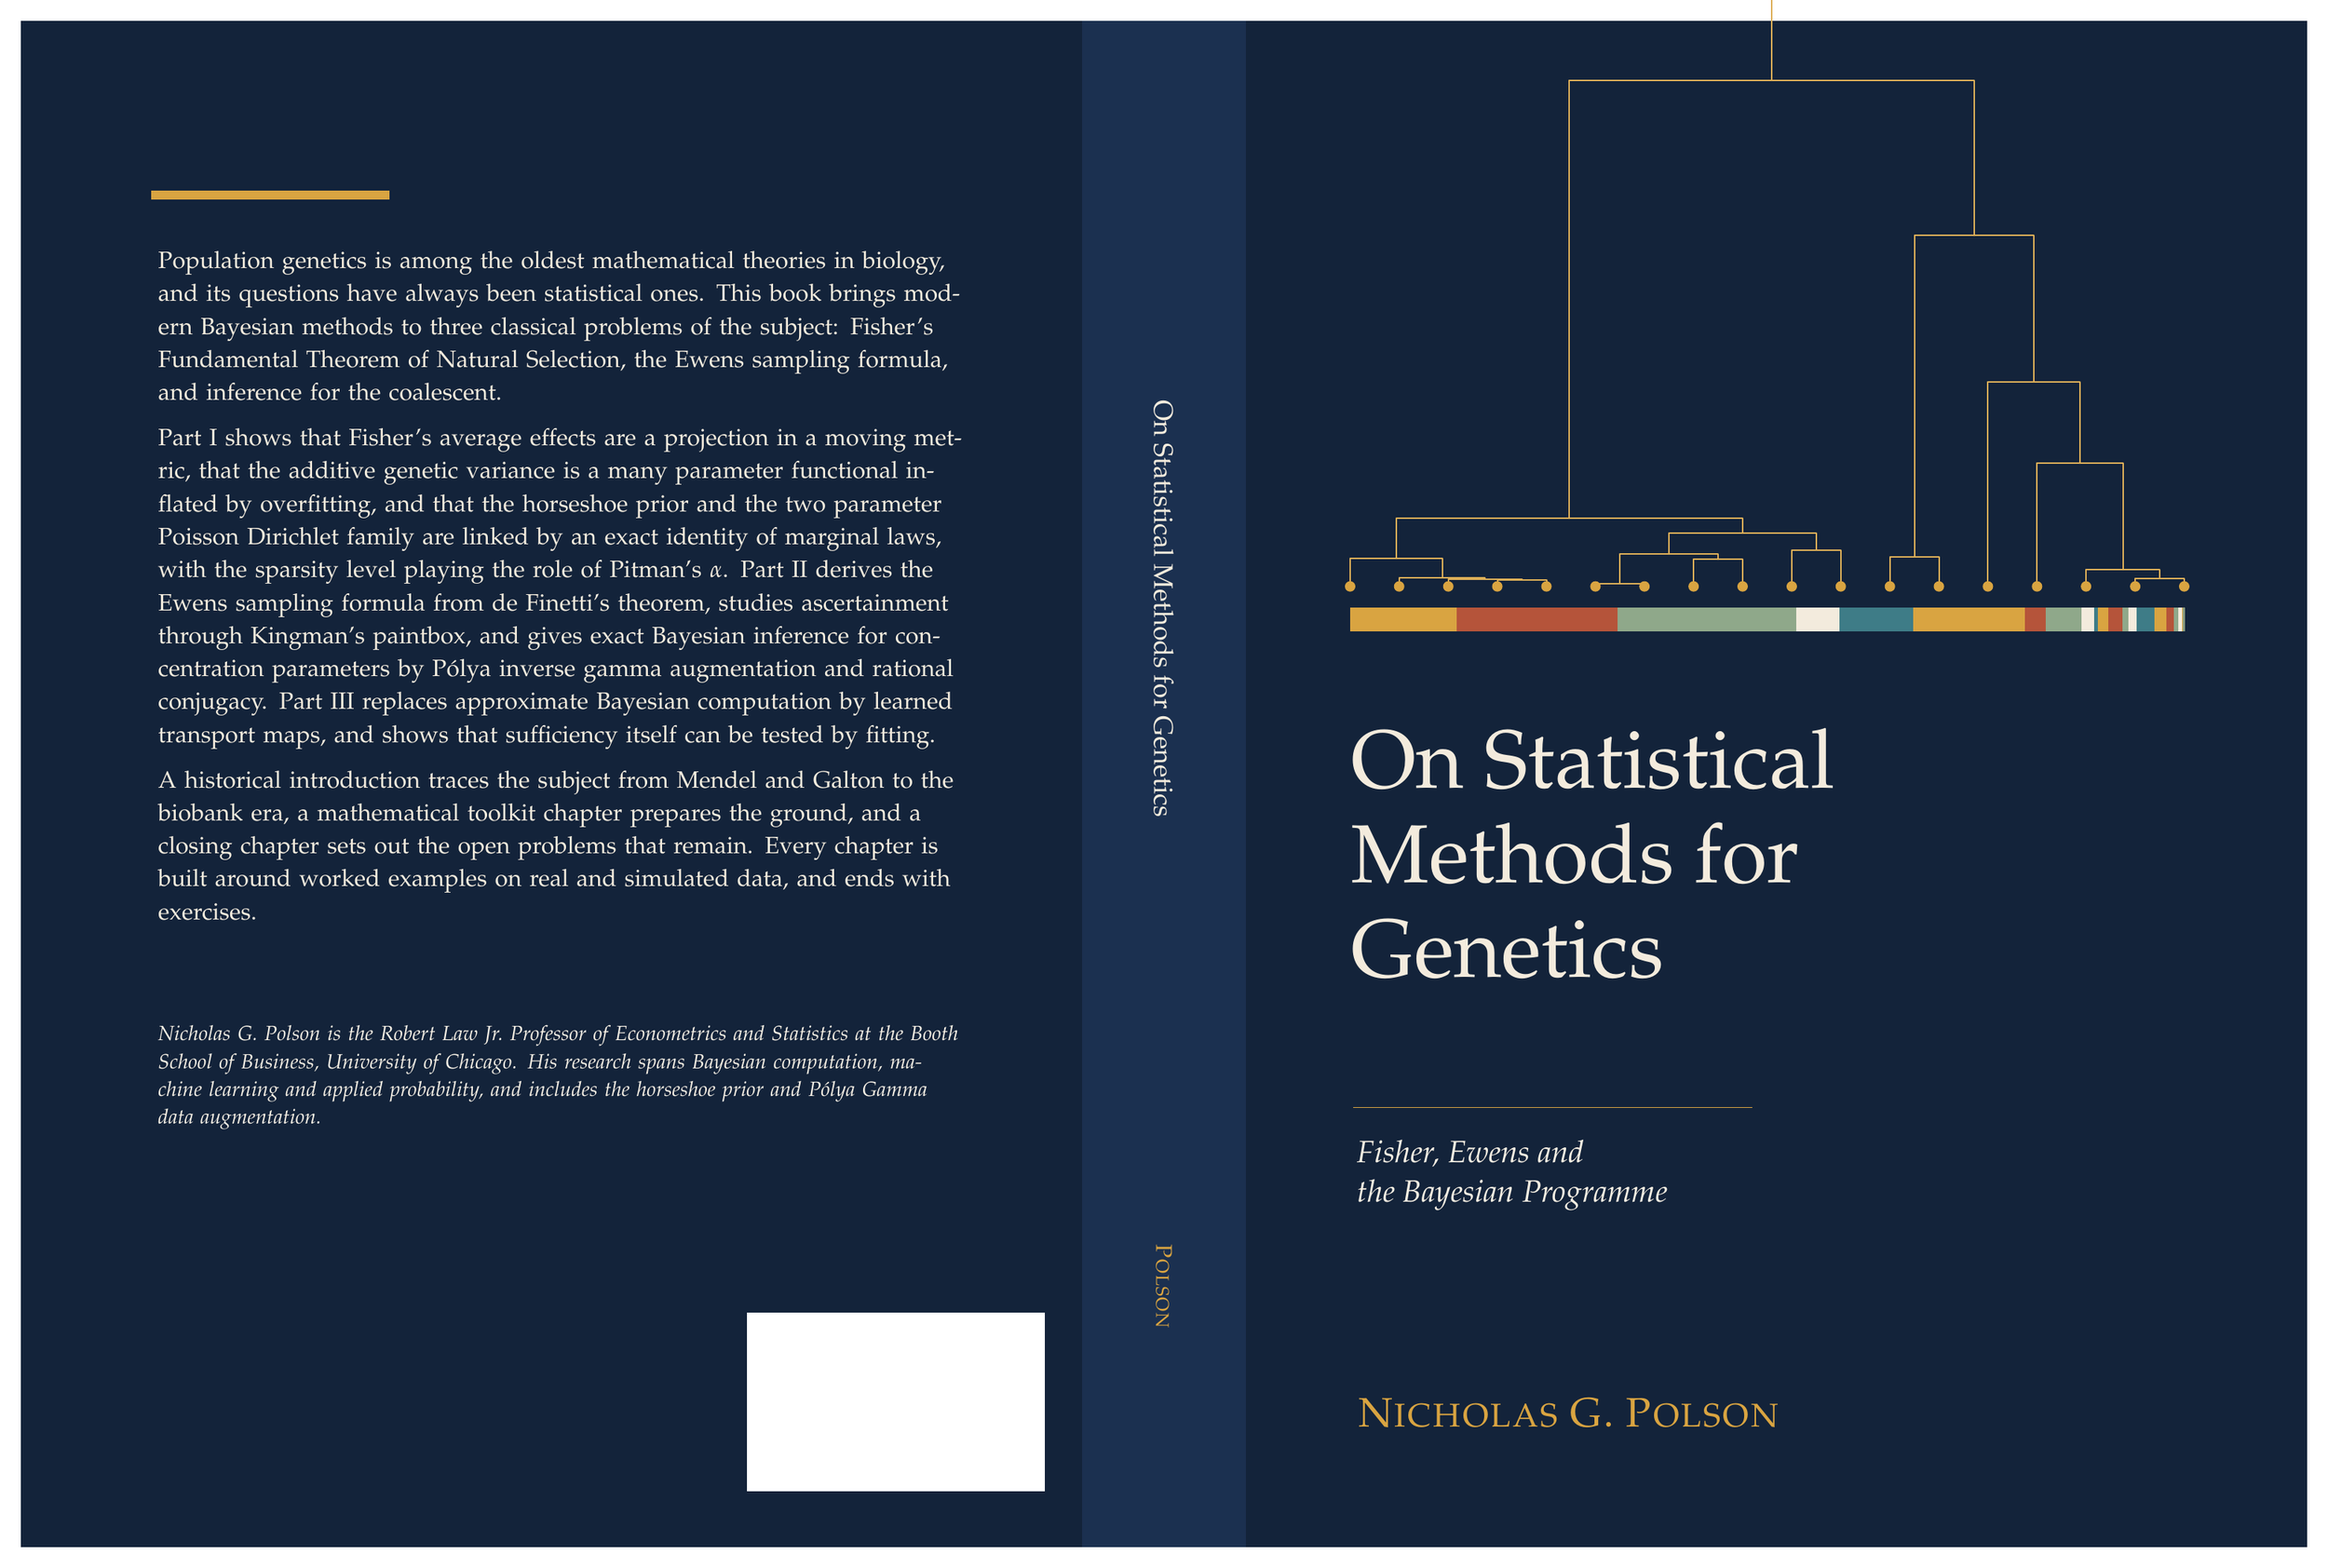
\begin{tikzpicture}[x=1in,y=1in]
  % geometry helpers (origin at lower left of the bleed box)
  \pgfmathsetmacro{\B}{0.125}
  \pgfmathsetmacro{\S}{\spinewidth}
  \pgfmathsetmacro{\W}{\B+7+\S+7+\B}
  \pgfmathsetmacro{\Hh}{10.25}
  \pgfmathsetmacro{\fx}{\B+7+\S}   % left edge of front cover
  \pgfmathsetmacro{\sx}{\B+7}      % left edge of spine
  \useasboundingbox (0,0) rectangle (\W,\Hh);
  \fill[navy] (0,0) rectangle (\W,\Hh);
  \fill[navyb] (\sx,0) rectangle (\sx+\S,\Hh);

  %% ---------------- front cover
  % coalescent tree, root at top
  \begin{scope}[shift={(\fx+0.70,6.45)}, yscale=-1]
    \draw[treeline] (2.306,-0.000) -- (2.306,-0.183) -- (2.471,-0.183);
\draw[treeline] (2.965,-0.000) -- (2.965,-0.243) -- (3.129,-0.243);
\draw[treeline] (0.659,-0.000) -- (0.659,-0.047) -- (0.906,-0.047);
\draw[treeline] (1.647,-0.000) -- (1.647,-0.020) -- (1.812,-0.020);
\draw[treeline] (3.624,-0.000) -- (3.624,-0.199) -- (3.788,-0.199);
\draw[treeline] (3.294,-0.000) -- (3.294,-0.243) -- (3.129,-0.243);
\draw[treeline] (4.612,-0.000) -- (4.612,-0.830) -- (4.900,-0.830);
\draw[treeline] (5.271,-0.000) -- (5.271,-0.054) -- (5.435,-0.054);
\draw[treeline] (2.635,-0.000) -- (2.635,-0.183) -- (2.471,-0.183);
\draw[treeline] (4.941,-0.000) -- (4.941,-0.113) -- (5.188,-0.113);
\draw[treeline] (0.329,-0.000) -- (0.329,-0.059) -- (0.618,-0.059);
\draw[treeline] (3.953,-0.000) -- (3.953,-0.199) -- (3.788,-0.199);
\draw[treeline] (5.600,-0.000) -- (5.600,-0.054) -- (5.435,-0.054);
\draw[treeline] (4.282,-0.000) -- (4.282,-1.375) -- (4.591,-1.375);
\draw[treeline] (0.988,-0.000) -- (0.988,-0.042) -- (1.153,-0.042);
\draw[treeline] (1.976,-0.000) -- (1.976,-0.020) -- (1.812,-0.020);
\draw[treeline] (1.318,-0.000) -- (1.318,-0.042) -- (1.153,-0.042);
\draw[treeline] (0.000,-0.000) -- (0.000,-0.189) -- (0.309,-0.189);
\draw[treeline] (1.812,-0.020) -- (1.812,-0.216) -- (2.141,-0.216);
\draw[treeline] (1.153,-0.042) -- (1.153,-0.047) -- (0.906,-0.047);
\draw[treeline] (0.906,-0.047) -- (0.906,-0.059) -- (0.618,-0.059);
\draw[treeline] (5.435,-0.054) -- (5.435,-0.113) -- (5.188,-0.113);
\draw[treeline] (0.618,-0.059) -- (0.618,-0.189) -- (0.309,-0.189);
\draw[treeline] (5.188,-0.113) -- (5.188,-0.830) -- (4.900,-0.830);
\draw[treeline] (2.471,-0.183) -- (2.471,-0.216) -- (2.141,-0.216);
\draw[treeline] (0.309,-0.189) -- (0.309,-0.458) -- (1.472,-0.458);
\draw[treeline] (3.788,-0.199) -- (3.788,-2.356) -- (4.190,-2.356);
\draw[treeline] (2.141,-0.216) -- (2.141,-0.360) -- (2.635,-0.360);
\draw[treeline] (3.129,-0.243) -- (3.129,-0.360) -- (2.635,-0.360);
\draw[treeline] (2.635,-0.360) -- (2.635,-0.458) -- (1.472,-0.458);
\draw[treeline] (1.472,-0.458) -- (1.472,-3.400) -- (2.831,-3.400);
\draw[treeline] (4.900,-0.830) -- (4.900,-1.375) -- (4.591,-1.375);
\draw[treeline] (4.591,-1.375) -- (4.591,-2.356) -- (4.190,-2.356);
\draw[treeline] (4.190,-2.356) -- (4.190,-3.400) -- (2.831,-3.400);
\draw[treeline] (2.831,-3.400) -- (2.831,-4.000);
\fill[gold] (2.306,0) circle (0.035);
\fill[gold] (2.965,0) circle (0.035);
\fill[gold] (0.659,0) circle (0.035);
\fill[gold] (1.647,0) circle (0.035);
\fill[gold] (3.624,0) circle (0.035);
\fill[gold] (3.294,0) circle (0.035);
\fill[gold] (4.612,0) circle (0.035);
\fill[gold] (5.271,0) circle (0.035);
\fill[gold] (2.635,0) circle (0.035);
\fill[gold] (4.941,0) circle (0.035);
\fill[gold] (0.329,0) circle (0.035);
\fill[gold] (3.953,0) circle (0.035);
\fill[gold] (5.600,0) circle (0.035);
\fill[gold] (4.282,0) circle (0.035);
\fill[gold] (0.988,0) circle (0.035);
\fill[gold] (1.976,0) circle (0.035);
\fill[gold] (1.318,0) circle (0.035);
\fill[gold] (0.000,0) circle (0.035);
  \end{scope}
  % paintbox strip under the tree
  \begin{scope}[shift={(\fx+0.70,6.15)}]
    \fill[gold] (0.0000,0) rectangle (0.7152,0.16);
\fill[rust] (0.7152,0) rectangle (1.7936,0.16);
\fill[sage] (1.7936,0) rectangle (2.9943,0.16);
\fill[cream] (2.9943,0) rectangle (3.2865,0.16);
\fill[teal] (3.2865,0) rectangle (3.7807,0.16);
\fill[gold] (3.7807,0) rectangle (4.5320,0.16);
\fill[rust] (4.5320,0) rectangle (4.6703,0.16);
\fill[sage] (4.6703,0) rectangle (4.9111,0.16);
\fill[cream] (4.9111,0) rectangle (4.9970,0.16);
\fill[teal] (4.9970,0) rectangle (5.0215,0.16);
\fill[gold] (5.0215,0) rectangle (5.0889,0.16);
\fill[rust] (5.0889,0) rectangle (5.1831,0.16);
\fill[sage] (5.1831,0) rectangle (5.2235,0.16);
\fill[cream] (5.2235,0) rectangle (5.2787,0.16);
\fill[teal] (5.2787,0) rectangle (5.4011,0.16);
\fill[gold] (5.4011,0) rectangle (5.4781,0.16);
\fill[rust] (5.4781,0) rectangle (5.5294,0.16);
\fill[sage] (5.5294,0) rectangle (5.5594,0.16);
\fill[cream] (5.5594,0) rectangle (5.5858,0.16);
\fill[teal] (5.5858,0) rectangle (5.5863,0.16);
\fill[gold] (5.5863,0) rectangle (5.5899,0.16);
\fill[rust] (5.5899,0) rectangle (5.5904,0.16);
\fill[sage] (5.5904,0) rectangle (5.5967,0.16);
\fill[cream] (5.5967,0) rectangle (5.5974,0.16);
\fill[teal] (5.5974,0) rectangle (5.5978,0.16);
\fill[gold] (5.5978,0) rectangle (5.5980,0.16);
\fill[rust] (5.5980,0) rectangle (5.5980,0.16);
\fill[sage] (5.5980,0) rectangle (5.5990,0.16);
\fill[cream] (5.5990,0) rectangle (5.5994,0.16);
\fill[teal] (5.5994,0) rectangle (5.5995,0.16);
\fill[gold] (5.5995,0) rectangle (5.5996,0.16);
\fill[rust] (5.5996,0) rectangle (5.5997,0.16);
\fill[sage] (5.5997,0) rectangle (5.5997,0.16);
\fill[cream] (5.5997,0) rectangle (5.5999,0.16);
\fill[teal] (5.5999,0) rectangle (5.5999,0.16);
\fill[gold] (5.5999,0) rectangle (5.5999,0.16);
\fill[rust] (5.5999,0) rectangle (5.5999,0.16);
\fill[sage] (5.5999,0) rectangle (5.6000,0.16);
\fill[cream] (5.6000,0) rectangle (5.6000,0.16);
\fill[teal] (5.6000,0) rectangle (5.6000,0.16);
\fill[gold] (5.6000,0) rectangle (5.6000,0.16);
  \end{scope}
  \node[anchor=north west, text=cream, align=left, font=\fontsize{40}{46}\selectfont]
     at (\fx+0.66,5.55) {On Statistical\\Methods for\\Genetics};
  \draw[gold, line width=0.6pt] (\fx+0.72,2.95) -- (\fx+3.4,2.95);
  \node[anchor=north west, text=cream!85, align=left, font=\fontsize{15}{19}\selectfont\itshape]
     at (\fx+0.70,2.78) {Fisher, Ewens and\\the Bayesian Programme};
  \node[anchor=south west, text=gold, font=\fontsize{20}{24}\selectfont\scshape]
     at (\fx+0.70,0.75) {Nicholas G.\ Polson};

  %% ---------------- spine (text reads top to bottom)
  \node[rotate=-90, text=cream, font=\fontsize{13}{15}\selectfont]
     at (\sx+0.5*\S,6.3) {On Statistical Methods for Genetics};
  \node[rotate=-90, text=gold, font=\fontsize{11}{13}\selectfont\scshape]
     at (\sx+0.5*\S,1.75) {Polson};

  %% ---------------- back cover
  \fill[gold] (\B+0.75,9.05) rectangle (\B+2.35,9.11);
  \node[anchor=north west, text width=5.4in, text=cream, align=left,
        font=\fontsize{11.5}{16}\selectfont] at (\B+0.75,8.75) {%
  Population genetics is among the oldest mathematical theories in biology, and its questions have always
  been statistical ones. This book brings modern Bayesian methods to three classical problems of
  the subject: Fisher's Fundamental Theorem of Natural Selection, the Ewens sampling formula, and
  inference for the coalescent.\par\medskip
  Part I shows that Fisher's average effects are a projection in a moving metric, that the additive
  genetic variance is a many parameter functional inflated by overfitting, and that the horseshoe
  prior and the two parameter Poisson Dirichlet family are linked by an exact identity of marginal
  laws, with the sparsity level playing the role of Pitman's $\alpha$. Part II derives the Ewens sampling formula from de Finetti's theorem, studies
  ascertainment through Kingman's paintbox, and gives exact Bayesian inference for concentration
  parameters by P\'olya inverse gamma augmentation and rational conjugacy. Part III replaces
  approximate Bayesian computation by learned transport maps, and shows that sufficiency itself
  can be tested by fitting.\par\medskip
  A historical introduction traces the subject from Mendel and Galton to the biobank era, a
  mathematical toolkit chapter prepares the ground, and a closing chapter sets out the open
  problems that remain. Every chapter is built around worked examples on real and simulated
  data, and ends with exercises.};
  \node[anchor=north west, text width=5.4in, text=cream!80, align=left,
        font=\fontsize{10}{13.5}\selectfont\itshape] at (\B+0.75,3.55) {%
  Nicholas G.\ Polson is the Robert Law Jr.\ Professor of Econometrics and Statistics at the Booth
  School of Business, University of Chicago. His research spans Bayesian computation, machine
  learning and applied probability, and includes the horseshoe prior and P\'olya Gamma data
  augmentation.};
  % barcode area kept clear (KDP places the barcode here)
  \fill[white] (\B+7-0.25-2.0,0.125+0.25) rectangle (\B+7-0.25,0.125+0.25+1.2);
\end{tikzpicture}
\end{document}
